% !TeX spellcheck = en_GB
%****************************************************
%	CHAPTER 3 - Map Merging
%****************************************************
\chapter{Map merging}
\label{sec:map-merging}
%----------------------------------------------------
This chapter discusses map merging for multiple robots; the discussion includes reviewing the literature and parameter tuning experiments. In multi-robot SLAM, two or more robots explore an environment independently and generate local partial maps. Merging of all the partial maps to form a global map, is functional to applications such as finding frontiers for all the robots in the environment \cite{Burgard2000}. Map merging can be simplified into two steps which involves finding alignments (such as rotation, resolution and translation) between maps, and then merging maps using information from the first step. The maps and other information about the robots are shared to find the alignment between the different maps in the steps mentioned. The focus, as mention in the previous chapter, is on merging 2D occupancy grid maps.

%====================================================
\section{Problem statement}
%----------------------------------------------------
Consider a large and complex environment, where a team of robots is tasked to maps different parts of an environment at different grid map resolutions. The resolution is defined by a metric $x$ per cell; in this work, we will be using meters/cell (m/cell), which is the size in meters of an individual grid map cell. The partially overlapping local grid maps generated from the task must be integrated into a global map that can be useful for robots to perform operations such as path planning and frontier finding.

\subsection{Definitions}

Definition 1: Let $\mathbf{m}$ be a map of $N$ by $M$, where $N$, $M$ are positive real numbers:

\begin{equation}
    \mathbf{m}: [0, N] \times [0, M] \rightarrow \mathbb{R}
\end{equation}

We can also denote a set of $N$ by $M$ maps as $\mathbf{I}_{N \times M}$


Definition 2:  According to \cite{Carpin2008b}, the goal of pairwise map merging is to find a relative transformation denoted by:

\begin{equation}
    \mathbf{T}_{t_x,t_y,\theta} = \begin{bmatrix}
            s\mathbf{R} & \mathbf{t}\\
            0 & 1
        \end{bmatrix}
        \label{eq:transformation}
\end{equation}

, where $s \in \mathbb{R}$ is the scale factor, $\mathbf{R} \in \mathbb{R}^{2\times2}$ represents a two-dimensional counterclockwise rotation matrix about origin point ($x,y$) of $\theta$ angle $\theta$ and $\mathbf{t} \in \mathbb{R}^2$ indicates a translation vector ($t_x, t_y$). More specifically, $\mathbf{R}$ and $\mathbf{t}$ can be denoted as follows:

\begin{equation}
    \mathbf{R} =  \begin{bmatrix}
        cos(\theta) & sin(\theta)\\
        -sin(\theta) & cos(\theta)
        \end{bmatrix},
    \mathbf{t} = \begin{bmatrix}
        t_x\\
        t_y
        \end{bmatrix}
\end{equation}

Definition 3:  
Let $\mathbf{m}_1, \mathbf{m}_2, \dots, \mathbf{m}_k$ be $k$ maps in $I_{N \times M}$
\begin{equation}
    \omega(\mathbf{m}_1, \mathbf{m}_2) = \sum_{i=0}^{N-1}\sum_{j=0}^{M-1} Eq(\mathbf{m}_1[i,j], \mathbf{m}_2[i,j]).
\end{equation}

Here $Eq(a,b)$ is one when a=b and zero otherwise, and $\omega$ is an overlapping function that measures how much the two maps agree. In an ideal world, robots would cover the same area, where there exists a transformation which yields $ \omega(\mathbf{m}_1, \mathbf{m}_2) = N \times M$. In the real world this is not the case, so the objective is to find the transformation which maximises overlap. Therefore, ${x, y, \theta}$-map transformation, $\mathbf{T}_{t_x,t_y,\theta}$ is determined by maximising $ \omega(\mathbf{m}_1, \mathbf{T}_{t_x,t_y,\theta}(m_2))$.

Suppose there are a couple of overlapping maps: the subject map $\mathbf{P}$ and the seed map $\mathbf{Q}$, which have different resolutions built by robots exploring two parts of the same environment. To merge the seed map $\mathbf{Q}$ into map $\mathbf{P}$, a transformation $\mathbf{T}_{t_x, t_y, \theta}(x, y)$ is applied to map $\mathbf{Q}$, to obtain new map $\mathbf{Q}^{'}$ indicated as $\mathbf{Q}^{'} = \mathbf{T}_{t_x, t_y, \theta}(x, y) \mathbf{Q}$. Once transformed map $\mathbf{P}$ and $\mathbf{Q}^{'}$ are then merged to form a global map. The following section explores solutions to solving the map merging problem defined in this section. 

\section{Related work}

Various solutions are presented in the literature for maps from a team of mobile robots. The following four cases, where most are discussed in \cite{Rone2013} are used to study map merging in this section:
 
\begin{enumerate}[a.]
	\item \textbf{Known initial configuration}: This case is the simplest as the initial pose of the robots is known, which simplifies the map alignment step. This assumption is a limited case as many times the initial poses are not known as described in \cite{Carlone2010a}. In the case of Figure \ref{fig:initial}, for the initial poses to be known, the relative pose would be described by the distance between $G_i$ and $G_j$.
	\item \textbf{Rendezvous}: This case is where two robots meet at a point such as in Figure \ref{fig:rendevous}, where the relative pose is calculated using methods such as line-of-sight measurement. The distance between the robots determines the accuracy at the meeting point and the method used to compute the relative distance. However, this adds a level of complexity to the system as either the robots need to coordinate a meeting point or use a method such as an image processing to recognise other robots \cite{4058636}.
	\item \textbf{Relative position estimation}: In this case, a robot localises other robots in its local map. The critical element to this case is that there is no need for the robots to rendezvous or have knowledge of initial relative positions \cite{1249654}.
	\item \textbf{Overlaps}: In this case, overlaps in the map are used to calculate the relative transformation between different maps such as in Figure \ref{fig:overlap}. The main challenge is finding the maps' overlaps using features such as doors, junctions or corners. The optimal algorithm is one that can identify both false and true matches, in the least amount of time with the highest accuracy \cite{Birk2006}.
\end{enumerate}

\begin{figure}[H]
    \centering
    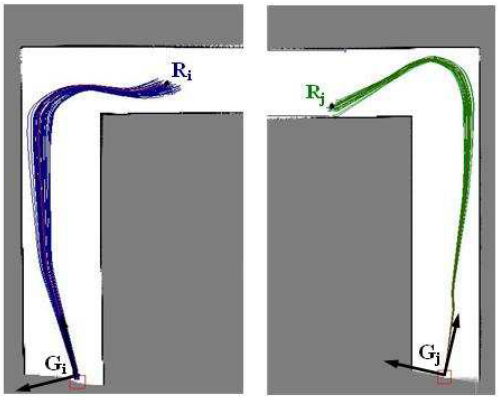
\includegraphics[width=0.5\textwidth]{figs/initial_configuration_example.png}
    \caption[Two relative robot maps]{This figure shows an example of two robots with unknown initial configurations. Each robot estimates both trajectory and map hypotheses in its own reference frame. In the case where initial configuration is known, the relative distance between $G_i$ and $G_j$ is known. Taken from \cite{Carlone2010a} }
    \label{fig:initial}
\end{figure}

\begin{figure}[H]
    \centering
    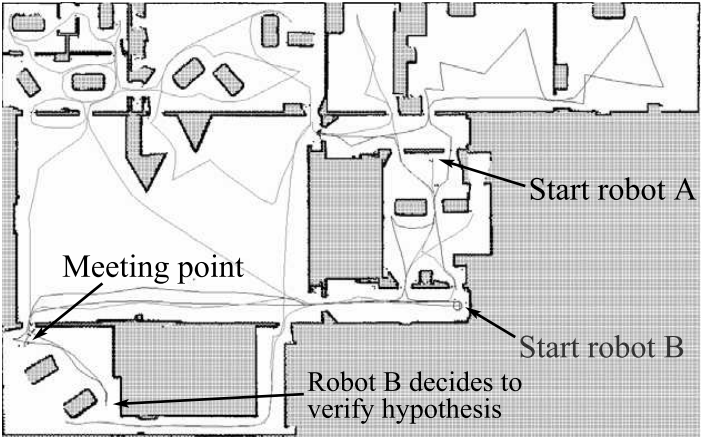
\includegraphics[width=0.5\textwidth]{figs/rendezvous_example.png}
    \caption[Example of coordinated exploration]{Example of a coordinated exploration of an unknown environment, from unknown locations. When then the robots meet at the meeting pint, they estimate and verify relative locations using a rendezvous approach. At the meeting point they share a map and their coordinate. Taken from \cite{Thrun2006}.}
    \label{fig:rendevous}
\end{figure}

\begin{figure}[H]
    \centering
    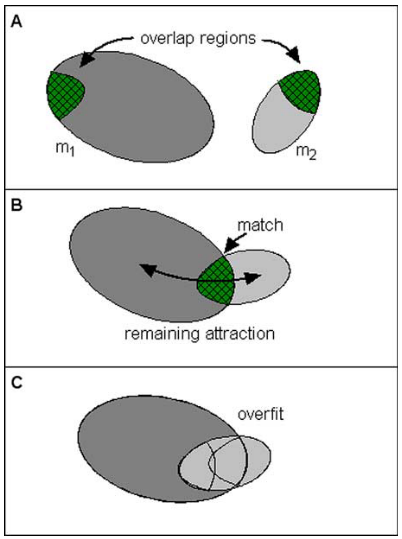
\includegraphics[width=0.5\textwidth]{UCT_MSc_Thesis/figs/overlap_example.png}
    \caption[Overlap matching example]{(A) describes the overlap region of the $m_1$ and $m_2$, where similarity is maximised. In (B) the identical regions are matched, where the unmatched regions remain unchanged. (C) is an example of over-fitting, where an area without a match is merged into another map. Taken from \cite{Birk2006}.}
    \label{fig:overlap}
\end{figure}


Early strategies of solving map merging with multiple robots such as \cite{Burgard2000} assume a known initial position of the robots. Although this method required minimal computational power, the method will fail if robots are unaware of each other's initial position. The more flexible approaches started presenting themselves in \cite{Carpin2005}, where map merging was solved as an optimisation problem. The authors in \cite{Carpin2005}, proposed a stochastic search approach to solve the problem. This method is an exhaustive approach based on adaptive random walks aiming to find suitable transformation to overlap the maps. Work was further done by \cite{Birk2006a} to improve the algorithm, and the improvement attempts to detect failures and guide the search to find the optimal solution. However, the exhaustive nature of the algorithm makes it computationally expensive to implement.

Xin Ma et al. later proposed a generic adaptive algorithm implemented without standard reference frames and relative pose information of robots \cite{XinMa2008}. The authors claim that their algorithm outperforms one presented by \cite{Carpin2005} because the generic adaptive algorithm can search the optimal match overlapping area more effectively. Avoiding premature convergence, low convergence speed and low stability. However, they did not present a merging of complex real-world maps, and the experimental results are of simple simulation maps. 

Saeedi et al. propose an artificial intelligence-based approach to map merging  \cite{Saeedi2011a}. The algorithm clusters the maps using neural-networks based on self-organised map (SOM); the cluster norms are used to find the relative transformation between the maps. Although this reduces dimensionality and improves processing time, the downfall is that some information is lost in the process. Dinnissen et al. proposed another artificial intelligence-based novel approach using reinforcement learning; the model is trained to determine a policy capable of deciding the best merge \cite{Dinnissen2012}. This approach allows the robot to incur less error during merging compared to simply merging after alignment. However, the model is validated using a simulated dataset instead of a real-world dataset.
 
Blanco et al. proposed a novel map-matching algorithm from image registration \cite{Blanco2013}. In this method, the maps are represented both as points and occupancy grid maps. The grid maps are firstly matched then the corresponding point maps are matched to help remove false matches. The transformation is determined by removing high-frequency noise and using feature detectors such as Harris or Kanade Lucas Tomasi (KLT). Matches are then filtered using a customised RANSAC algorithm based on the sum of Gaussian distributions. Based on the experimental results, this method deals adequately with uncertainty and ambiguity when matching maps.

Alternatively, Hough transforms are a way of representing geometrical data within maps. \cite{Carpin2008} proposes a Hough spectrum-based approach which was first introduced by \cite{1570528}. The maps are transformed into the Hough space, and the resulting Hough images are then correlated to find the potential transformations (rotation/translation). The authors introduce an acceptance index which tells how well-aligned maps are for each transformation. This index has values between 0 and 1, where 1 is a correct transformation, and 0 is an incorrect transformation. However, this solution fails when there is not enough overlap between maps. \cite{Saeedi2014c} further improved the approach by adapting the new cross-correlation operator allowing the algorithm to deal with less overlap in the maps.

Topology is a field of mathematics that studies the properties preserved through stretching, deforming, and twisting of an object \cite{Kuipers1991}. Topologies can be used in mapping to abstract objects while ignoring details. Topological maps can use a graph to represent navigation possibilities through an environment, where vertices are ``places'' and edges represent paths between the``places''. Even though maps can lose information from this abstraction, it can improve communication and mutual perception. Topological approaches have applications in map merging such as \cite{Huang2005a, Saeedi2012a }. 

Huang et al. proposed a topological approach which uses both structural and geometrical attributes of the Voronoi graph, to determining best correspondence between maps with overlapping areas\cite{Huang2005a}. The topological map is built on the occupied space instead of using free space because the assumption is that robots will be able to recognise the area of the map that correspond to vertices. The limitations of this method are that the maps are not updated. Saeedi et al. proposed a probabilistic topological representation, the essential to add probabilistic information to generalised Voronoi diagram \cite{Saeedi2012a}. They refer to the method as probabilistic generalised Voronoi diagram (PGVD). The method is used to match parts of the map, which are more specific, therefore improving the reliability of finding relative transformation between maps and fusing them.

All the strategies mentioned above are only merging grid maps that have the same resolution. However, there is a need for representing maps with multiple resolutions for building large scale maps. Some areas of a large scale environment may include more details than others. Therefore for reasons of compactness, the map can be built at a fine resolution in areas of more details, and at a coarse resolution in areas with fewer details\cite{Wurm2010OctoMapA}. In \cite{Ma2016}, map merging is approached as a unique image registration case. The solution considers non-common areas and an objective function based on the trimmed mean-square error (MSE) is designed. The objective function is then solved using a trimmed and scaling iterative closest point (TsICP) algorithm. The TsICP algorithm needs a good initial transformation to converge locally. Therefore the initial transformation is obtained by extracting scale-invariant feature transform (SIFT) features, and then the random sample consensus (RANSAC) algorithm is used to find geometrically consistent features matched. The results presented show that this algorithm is more accurate and robust compared to \cite{Blanco2013} and \cite{Carpin2008}'s approach.

Further sections will discuss the use of image registration as a solution to multi-resolution map merging.

%====================================================
\section{Image registration approach}
%----------------------------------------------------

As mentioned in the review above, map merging can be view as an image registration problem. For a pair of occupancy grid maps, features are extracted, matched, and then aligned and merged to give a global grid map. This section will discuss the following topics of image registration: feature detection, matching, and alignment. 

%Occupancy grids acquired from mapping are smaller than megapixel images from cameras even for large maps; hence merging time is reasonable. Furthermore, occupancy girds have fewer features than camera photos, making merging more difficult and less accurate. However, this depends on the feature detection method used. An online merging process can be run at lower frequencies even if the map is updated at a higher frequency, and this can be achieved by using previously estimated transformation between maps, which can further reduce estimation time. In many cases, transformations can change only in the initial phases of mapping, once there is enough overlap between maps transformations can be estimated with high precision. Allowing for re-estimation at even lower frequencies, if map quality is high. This section will discuss the following topics of image registration: feature detection, matching, and alignment. 

%====================================================
\subsection{Feature detection}
%----------------------------------------------------

The process of abstracting an image is called feature detection. The abstraction is computed by deciding at every point of the image if there is a feature based on a set of rules. Features have no universal definition and depend on the application, and a feature is usually defined as a region of ``interest'' within an image. Features can be specific structures such as points, edges, corners or objects. Ideally, the detection of features should be robust to transforms (rotation, scale, illumination, noise and affine transformation) in an image, with distinctive features to be matched with high probability. 

The main components of feature detection are:

%....................................................
\begin{itemize}
    \item \textbf{Region of Interest:} This is a point or region which is expressive in appearances such as corner, edge and objects. This interest region is usually stable to: rotation, scale, illumination, noise and affine transformation.
%----------------------------------------------------
    \item \textbf{Descriptor:} This is the local appearance around each region of interest, which is ideally described in a way that is invariant to: rotation, scale, illumination, noise and affine transformation. Typically each region of interest will have a unique descriptor. 
%----------------------------------------------------
\end{itemize}
%....................................................

Once features have been identified and described, they can be applied to image-stitching processes, where features from multiple partial images are matched to align and merge the images to form a single picture. This section will further discuss three scale-invariant feature detection methods (SIFT, SURF and ORB).

\textbf{Scale Invariant Feature Transform (SIFT)} is a feature detector developed by Lowe in 2004 \cite{Lowe2004}. SIFT solves image rotation, affine transformations, intensity, and viewpoint change in matching features. The SIFT algorithm employs four basic steps:

%....................................................
\begin{enumerate}
%----------------------------------------------------
\item \textbf{Estimate of scale-space extrema:} Some objects are only detectable at specific scales. For example, if zoomed into the eye's pupil, one might mistake it for a flower or other object, however, if zoomed out to the point of seeing their eyebrows one will realise that it is an eye pupil. SIFT recognises this attribute in nature and attempts to replicate the effect by using scale-space filtering. The scale-space of an image is represented by $L(x, y, \sigma)$, where $(x, y)$ is a potentially key-point location and $\sigma$ is the scaling parameter. In the scale-space filtering, Laplacian of Gaussian (LoG) is found for the image at various $\sigma$ values so that we can find local maxima across various scales and the space of the image. This LoG is computationally costly; therefore, the Difference of Gaussian (DoG) is used instead. The DoG is obtained as the difference of Gaussian blurring of the image at different scales. The scale-space is divided into octaves, and the number of octaves is dependent on the original image size, see Figure \ref{fig:sift_steps}.
%----------------------------------------------------
\item\textbf{Finding key points:} Once key-point location candidates are localised from the previous step. They are refined by eliminating the low contrast points. A Taylor series expansion of the scale-space is used to get a more accurate extrema location, and if the intensity at this extrema is less than a set threshold, it is rejected.
\item \textbf{Orientation assignment:} Since we already know at which scale a key-point was detected, we have achieved scale in-variance. An orientation is assigned to key points to achieve invariance to image rotation, based on a local image gradient. A neighbourhood is taken around the key-point depending on the scale, and a gradient magnitude and direction is computed in this region.
%----------------------------------------------------
\item\textbf{Key-point descriptor:} So far a location, scale and orientation has been assigned to each key-point identified. Next, a key point descriptor is generated to compute the local image descriptor for each key-point based on image gradient magnitude and orientation. Ensuring that the key-point is highly distinctive to changes such as viewpoint and illumination. A neighbourhood around 16$\times$16 is taken around the key-point and then divided into sub-regions of 4$\times$4. An eight bin orientation histogram is created around each sub-region, making 128 bin values available. These 128 bin values are represented as a feature vector to form the key-point descriptor for each key-point. To further improve the descriptor, the key-points rotation is subtracted from each orientation and achieved illumination independence, and large numbers are thresholded.
%----------------------------------------------------
\end{enumerate}
%....................................................


SIFT has been proven to be very useful in mainly object recognition applications; however, it requires large computational complexity \cite{Lowe2004, karami2017image}. Several variants and extensions of SIFT improve the computational complexity \cite{Guzel2015, 6507640, 1315206}.

%....................................................
\begin{figure}[H]
%----------------------------------------------------
    \centering
%----------------------------------------------------
    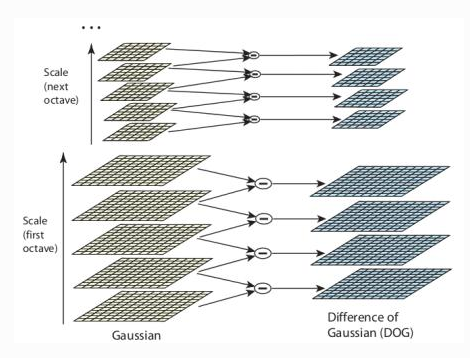
\includegraphics[width=0.5\textwidth]{UCT_MSc_Thesis/figs/sift_steps.png}
%----------------------------------------------------
    \caption[SIFT Difference of Gaussian]{Shown on the left are scale-space images produced by convolving the initial image with Gaussians repeatedly for each octave. The difference-of-Gaussian (DoG) images on the right are produced by subtracting adjacent Gaussian images. The Gaussian image is down-sampled by two after each octave, and then the process is repeated. Taken from \cite{Lowe2004}.}
%----------------------------------------------------
    \label{fig:sift_steps}
\end{figure}
%....................................................

\textbf{Speed up Robust Feature (SURF)} is the feature detector technique, which is an approximation of SIFT. The algorithm performs fast computation operations using box filters, thus enabling real-time applications such as object recognition \cite{BAY2008346}. SURF approximates the LoG with box filters, the advantage being that convolution with box filter can be easily calculated with the assistance of image integrals. Squares are used for approximation instead of Gaussian averaging because convolution with a square is faster than an image's integral. Furthermore, the estimation can be performed in parallel, the following Figure \ref{fig:surf_approximation} shows such an approximation. 

%....................................................
\begin{figure}[H]
%----------------------------------------------------
    \centering
%----------------------------------------------------
    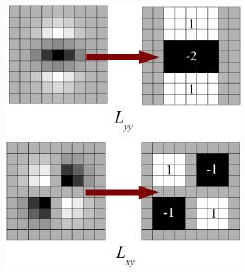
\includegraphics[width=0.5\textwidth]{UCT_MSc_Thesis/figs/surf_approximation.png}
%----------------------------------------------------
    \caption[Laplacian of Gaussian (LoG)]{Approximation of Laplacian of Gaussian (LoG) with Box Filter, where the grey regions are equal to zero.  Taken from \cite{BAY2008346}.}
%----------------------------------------------------
    \label{fig:surf_approximation}
\end{figure}
%....................................................

SURF relies on the determinant of the Hessian matrix for both scale and location of key-points. To find the key-points' orientation, SURF uses wavelets responses in both horizontal and vertical directions for a neighbourhood of size 6s and then applying Gaussian weights. They are then plotted as shown in Figure \ref{fig:surf_orientation}, where the red arrow is the dominant orientation, computed by summing of all the responses within a sliding orientation window. 

%....................................................
\begin{figure}[H]
    \centering
%----------------------------------------------------
    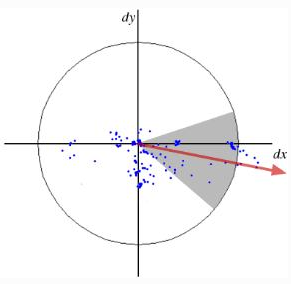
\includegraphics[width=0.5\textwidth]{UCT_MSc_Thesis/figs/surf_orientation.png}
%----------------------------------------------------
    \caption[Surf wavelet responses]{SURF uses wavelets responses in both horizontal and vertical directions then applying Gaussian weights, where the red arrow is the dominate orientation, computed by summing of all the responses within a sliding orientation window. Taken from \cite{BAY2008346}.}
%----------------------------------------------------
    \label{fig:surf_orientation}
%----------------------------------------------------
\end{figure}
%....................................................

Feature descriptor is achieved by again using wavelet responses in horizontal and vertical direction around a neighbourhood of size 20$\times$20 around the key-point, which is then divided into sub-regions of size 4$\times
$4 and then for each sub-region the wavelet responses are taken and represented to get SURF feature descriptor. SURF allows faster matching by using the sign of the Laplacian which is already computed by the detection, the sign distinguishes bright blobs on a dark background, which in case of matching the features are compared if they have matching contrast.

\textbf{Oriented FAST and Rotated BRIEF (ORB)} was developed at OpenCV labs as an alternative to SIFT and SURF. ORB fuses the well-known Features from Accelerated and Segments Test (FAST) key-point detector and BRIEF descriptor with modification to enhance performance \cite{Rublee2011}. 

FAST key-points are identified by comparing the brightness of 16 pixels surrounding a specific pixel, $p$. The pixels are then sorted into three categories lighter than $p$, darker than $p$ or similar to $p$. If more than eight of surrounding pixels are darker or brighter than $p$, then $p$ is selected as a key-point. Therefore, FAST key-points determine edges in the image. FAST key-point is, however, not an orientation and scale-invariant.

Similarly to SIFT, ORB identifies features at multiple scales, by using pyramids and representing the image at multiple scales. Change in intensity around the key-point is used to identify the orientation of the key-point. The intensity weighted centroid of the patch with located key-point (edge) at centroid is computed, to detect the change in intensity. The vector from the edge to centroid gives the orientation.

To compute the BRIEF descriptor, the algorithm takes all the key-points already found and converts them in binary feature vectors. In BRIEF, each key-point descriptor is defined by a feature 128 dimension vector, which as a floating-point number is 512 bytes. To prevent sensitivity to high-frequency noise, BRIEF begins by smoothing the image using a Gaussian kernel. Followed by selecting a pair of pixels in a defined neighbourhood of some height and width around the key-point. The first pixel is randomly selected from a Gaussian distribution centred around the key-point. Then the second on is randomly selected from a Gaussian distribution centred around the first pixel. If the first pixel is brighter than the second, a one is assigned else a zero. For a 128 dimension vector, this process is repeated 128 times, for each key-point. Given that BRIEF is not orientation invariant, ORB employs Rotation-aware BRIEF, by ``steering'' BRIEF descriptor in the key-point direction.

SIFT, SURF and ORB describe a feature with a key-point and a descriptor. In the next section, matching these features from images with partial overlap is discussed, followed by merging the images.

%====================================================
\subsection{Image matching}
%----------------------------------------------------

The features detected in the map images need to be matched with high accuracy to get the best transformation (scaling, translation and rotation). The features are matched from one map to another using either a Brute-Force matcher or Fast Library for Approximate Nearest Neighbors (FLANN) Matcher provided by OpenCV. Brute-Force matcher uses the distance between features of the map to another and finds the closest one. Different distance measurements can be used with this matcher, depending on the feature detector. It is recommended to use the Euclidean distance for SIFT and SURF, and Hamming distance binary string based descriptors such as ORB, BRIEF and BRISK \footnote{https://opencv-python-tutroals.readthedocs.io/en/latest/py\_tutorials/py\_feature2d/py\_matcher/py\_matcher.html}. FLANN stands for Fast Library for Approximate Nearest Neighbours, and it is optimised for large datasets and high dimensional features. However, FLANN Matcher is not necessary for this application.

%====================================================
\subsection{Matching features}
%----------------------------------------------------

Brute-Force Matcher is used to matching features between two different images. Given that features (key-points and descriptors) have been identified, Brute-Force Matcher takes descriptors from each image and matches them using a distance calculation to determine the closest feature.

Different distance calculations can be using, euclidean distance is recommended for SIFT and SURF, and hamming distance is recommended for ORB \cite{itseez2015opencv}.

Euclidean distance is defined as the absolute value distance between two coordinates and is described as:

%....................................................
\begin{equation}
%----------------------------------------------------
    d(p,q) = \sqrt{(p - q)^2}
%----------------------------------------------------
\label{eq:euclidean_distance}
\end{equation}
%....................................................

Where, $p, q$ are two coordinates on a line. 

On the other hand, Hamming distance is a metric for comparing binary data strings. As discussed in the previous section, ORB produces binary descriptors, which are compared with an XOR operation. After XORing the two values, the total number of 1s is counted, which is the Hamming distance. The smaller the number of 1s, the smaller the Hamming distance.

%====================================================
\subsection{Map alignment}
%----------------------------------------------------
\label{subsec:map_alignment}

Even though maps may have a large number of matches between them, there will be outliers present. These outliers can cause some possible errors while aligning, which may affect the result. 

To remove outliers, algorithms such as Random sample consensus (RANSAC) or LEAST\_MEDIAN (LMEDS) are used so that good matches which provide correct estimation can be used. These good matches are called inliers, and remaining outliers are removed. OpenCV's \textbf{estimateAffinePartial2D()} has been used to remove outliers and estimate the transformation matrix $T_{t_x, t_y, \theta}$, defined by Equation \ref{eq:transformation} earlier.

This method (\textbf{estimateAffinePartial2D()}) has the following parameters:
%....................................................
\begin{itemize}
%----------------------------------------------------
\item \textbf{method}:	Robust method used to compute transformation. The following methods are possible, RANSAC and LMEDS.
%----------------------------------------------------
\item \textbf{ransacReprojThreshold}:  Maximum re-projection error in the RANSAC algorithm to consider a point as an inlier.
%----------------------------------------------------
\item \textbf{maxIters}: The maximum number of robust method iterations.
%----------------------------------------------------
\item \textbf{confidence}: Confidence level, between 0 and 1, for the estimated transformation.
%----------------------------------------------------
\end{itemize}
%....................................................

RANSAC was used, RANSAC is a robust estimation iterative procedure that uses a minimal set of randomly sampled correspondences to estimate image transformation parameters, and finds a solution that has the best consensus with the data \cite{Fischler1981}. The parameter value of confidence has been selected to be $0.99$ to achieve high accuracy and $ransacReprojThreshold$, and $maxIters$ will be discussed later.

The transformation $T$ from Equation \ref{eq:transformation}, can now be used to align the one image to match the other. An affine transformation fixed to rotation, translation and scaling transformations is used. Affine transformations can also do the following transformation: identity, reflection and shear but these do not apply to this thesis.

%\subsection{Merging}

%To remove the uncertainty of the estimated to transformation, known information from the map metadata is used. Each Occupancy Grid in the Robotic Operating System (ROS) has the metadata presented in Figure \ref{fig:metadata}. The resolution of each map can determine the scaling factor expected from $T$ if the scaling factors match the transformation is deemed successful, and the maps are then merged.

%\begin{figure}[H]
%    \centering
%    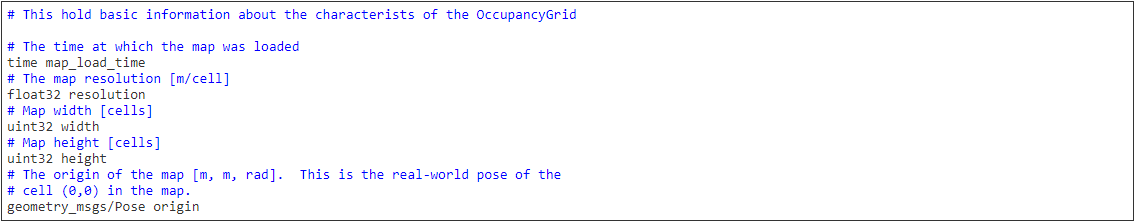
\includegraphics[width=1\textwidth]{figs/metadata_information.png}
%    \caption[Occupancy grid Metadata ROS Message]{Occupancy grid Metadata ROS Message, which is received with each %occupancy grid Map.}
%    \label{fig:metadata}
%\end{figure}


%\begin{figure}[H]
%   \centering
%    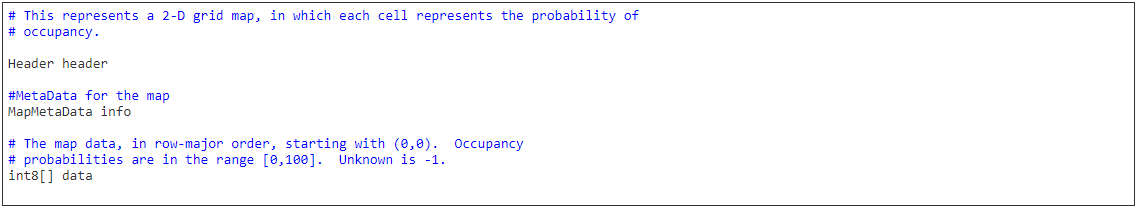
\includegraphics[width=1\textwidth]{figs/occupancy_grid_information.png}
%    \caption[Occupancy grid ROS Message]{Occupancy grid ROS Message, where data is an array describing the map and mapMetaData being the information about the map shown in Figure \ref{fig:metadata}}
%    \label{fig:occupancygridmsg}
%\end{figure}

%====================================================
\subsection{Method selection}
%----------------------------------------------------
\label{sub:sec:method}

Paper \cite{Karami2015}, investigates the sensitivity of SIFT, SURF, and ORB against intensity, rotation, scaling, shearing, fish-eye distortion, and noise. The investigation is general, and in the case of the work done in this thesis, further investigation is required for occupancy grid maps. This section investigates SIFT, SURF, and ORB's sensitivity against each rotation, scaling, translation, and noise, not includes in shearing and fish-eye distortion, which are not of interest in 2D occupancy grid maps, due to how they are generated. Open Source Computer Vision Library (OpenCV) \footnote{http://opencv.org}, which is an open-source BSD-licensed library that includes several hundred computer vision algorithms, is used for the image registration in this thesis.

In Figure \ref{fig:maps} are the maps used to test the robustness of the feature detection methods. These maps were produced in a real-world environment at the University of Cape Town due to work done in this thesis\footnote{Data-sets: \url{https://drive.google.com/drive/folders/1c\_2-T8FcrSmE0VDyHw20-jRLHKRuAvpE}}\footnote{GitHub repository: \url{https://github.com/dikokob/DikokoMScEng}}. The maps were produced using Hector-SLAM which each robot will be equipped with, and these maps are partial maps of the same area. The data used is later discussed in Chapter \ref{ch:experimental}.

%....................................................
\begin{figure}[H]
%----------------------------------------------------
    \centering
%----------------------------------------------------
    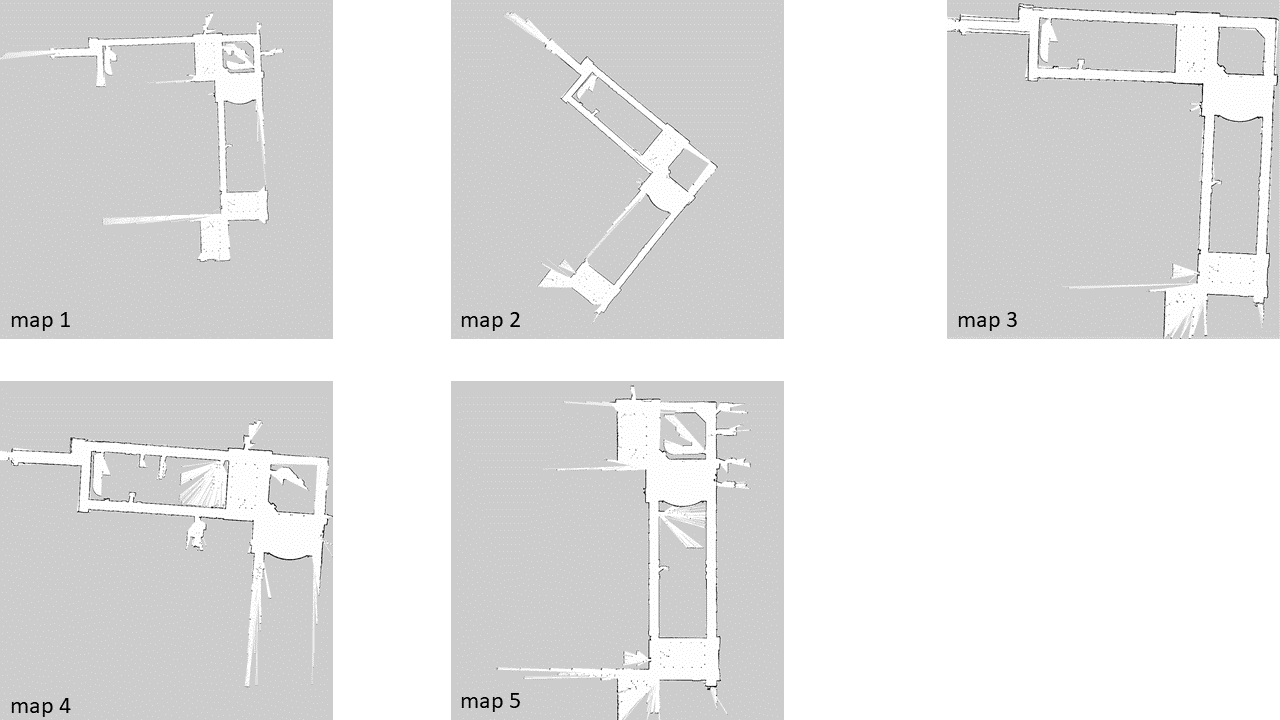
\includegraphics[width=1\textwidth]{figs/feature_images.png}
%----------------------------------------------------
    \caption[Occupancy grid map examples of a large indoor environment]{The following maps are of a large indoor environment used to test the robustness of the feature detection methods. The maps are produced using hector slam with a resolution of 0.5 m/cell. The generation of the maps are discussed in further details in Chapter \ref{ch:experimental}.}
%----------------------------------------------------
    \label{fig:maps}
%----------------------------------------------------
\end{figure}
%....................................................

A match ratio is used to investigate rotation, translation, scaling and noise sensitivity. The match ratio is calculated by

%....................................................
\begin{equation}
%----------------------------------------------------
    \frac{matches}{\min(num\_features\_orignal, num\_features\_mod)}
%----------------------------------------------------
    \label{eg:nmatch_ratio}
%----------------------------------------------------
\end{equation}
%....................................................

Where $num\_features$ is the number of features, and $matches$ is the number of matches found between the original and modified map features, using the earlier discussed Brute-Force matcher. The higher the match ratio, the more matches were found between the two maps. Note that in the investigations \textit{Kpnts1} are key-points from the original map and \textit{Kpnts2} are key-points from the modified map.

%====================================================
\subsubsection{Number of features}
%----------------------------------------------------

SIFT, SURF and ORB each produce a certain amount of features based on the algorithms. Figure \ref{fig:featuremaps} shows the features with descriptors shown by the feature's size and direction by the line within the circle. SIFT and ORB have a similar number of features whereas SURF has almost ten times more features, shown in \ref{table:numfeatures}. The number of features detected impacts the time cost of the process, more specifically the matching process. Also to be noted in Figure \ref{fig:featuremaps}, most of the ORB features are on the corners due to the nature of the algorithm and SIFT, and SURF features are highly variable size and location.

%....................................................
\begin{figure}[H]
%----------------------------------------------------
    \centering
%----------------------------------------------------
    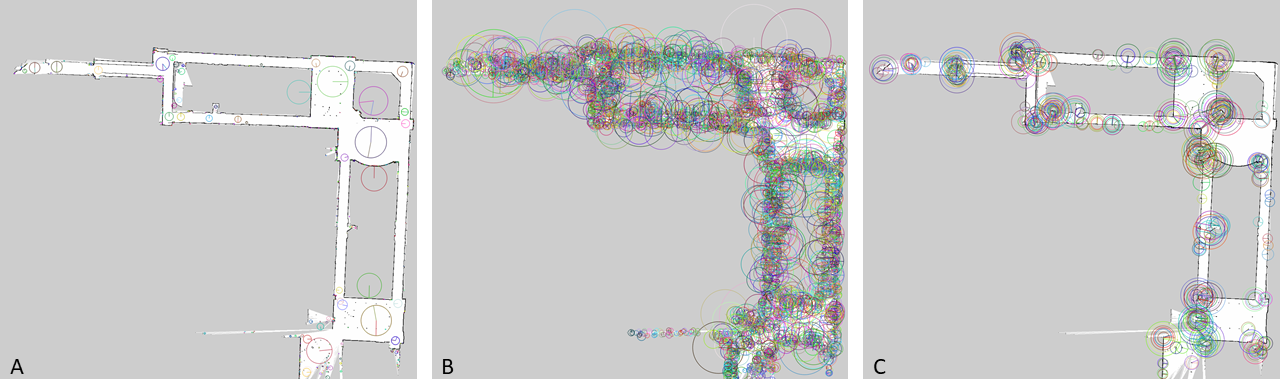
\includegraphics[width=1\textwidth]{figs/feature_maps.png}
%----------------------------------------------------
    \caption[Features detected on map3]{Features detected on $map_3$ from Figure \ref{fig:maps} where A) SIFT, B) SURF and C) ORB. See \footnote{https://github.com/dikokob/DikokoMScEng} for raw data. }
%----------------------------------------------------
    \label{fig:featuremaps}
%----------------------------------------------------
\end{figure}
%....................................................

%....................................................
\begin{table}[H]
%----------------------------------------------------
\centering
\caption{Average number of detected features (SIFT, SURF and ORB) of maps 1-5 in Figure \ref{fig:maps}.}
%----------------------------------------------------
%----------------------------------------------------
\begin{tabular}{ | m{3em} | m{2cm} | m{1.5cm} | m{1.5cm} | m{1.5cm} | m{3cm} | } 
%----------------------------------------------------
\hline
%----------------------------------------------------
\textbf{Maps} & \textbf{ORB}  & \textbf{SIFT} & \textbf{SURF} & \textbf{Total}\\ 
%----------------------------------------------------
\hline
%----------------------------------------------------
\textbf{map 1}  & 501 & 492 & 4291 & 5284 \\ 
%----------------------------------------------------
\hline
%----------------------------------------------------
\textbf{map 2}  & 500 & 528 & 3786 & 4814 \\ 
%----------------------------------------------------
\hline
%----------------------------------------------------
\textbf{map 3}  & 500 & 530 & 4503 & 5533 \\ 
%----------------------------------------------------
\hline 
%----------------------------------------------------
\textbf{map 4}  & 500 & 505 & 4224 & 5229 \\ 
%----------------------------------------------------
\hline 
%----------------------------------------------------
\textbf{map 5}  & 500 & 539 & 3282 & 4321 \\ 
%----------------------------------------------------
\hline 
%----------------------------------------------------
\end{tabular}
%----------------------------------------------------
\label{table:numfeatures}
%----------------------------------------------------
\end{table}
%....................................................

%\begin{figure}[H]
%    \centering
%    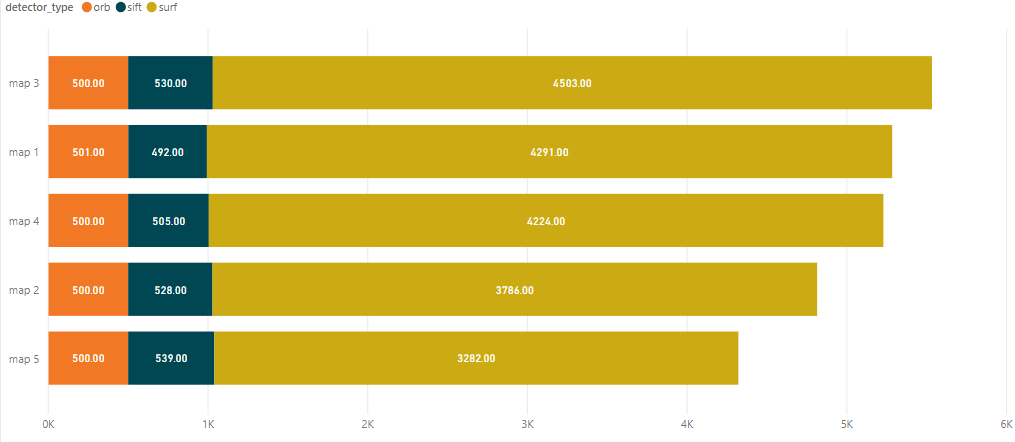
\includegraphics[width=1\textwidth]{figs/Number_of_Features.png}
%    \caption[Average number of features detected on each map using SIFT, SURF and ORB]{Average Number of Features detected on $map_{1-5}$ using different SURF, SIFT and ORB detection methods. }
%    \label{fig:numfeatures}
%\end{figure}

%====================================================
\subsubsection{Rotation}
%----------------------------------------------------

In this investigation, $map_3$ is rotated in steps of 30 degrees. The rotated map is matched with the original map. The results are shown in Figure \ref{fig:rotation} and Table \ref{table:rotation} are of $map_3$ rotated, where ORB is the fastest, followed by SIFT and SURF being the slowest. SIFT also has the highest match ratio, followed by ORB, with the lowest match ratio.

Table \ref{table:rotationangle} shows the match ratio versus the rotation angle, where rotation 0, 90 and 180 degrees ORB and SURF have the highest match ratio. However, they do not perform as well for other angles. The best overall performing feature detector is SIFT with an average of 0.90 match ratio, with SURF being the worst-performing. Also to be noted is that angles 0, 90 and 180 performed the best overall.

%....................................................
\begin{figure}[H]
%----------------------------------------------------
    \centering
%----------------------------------------------------
    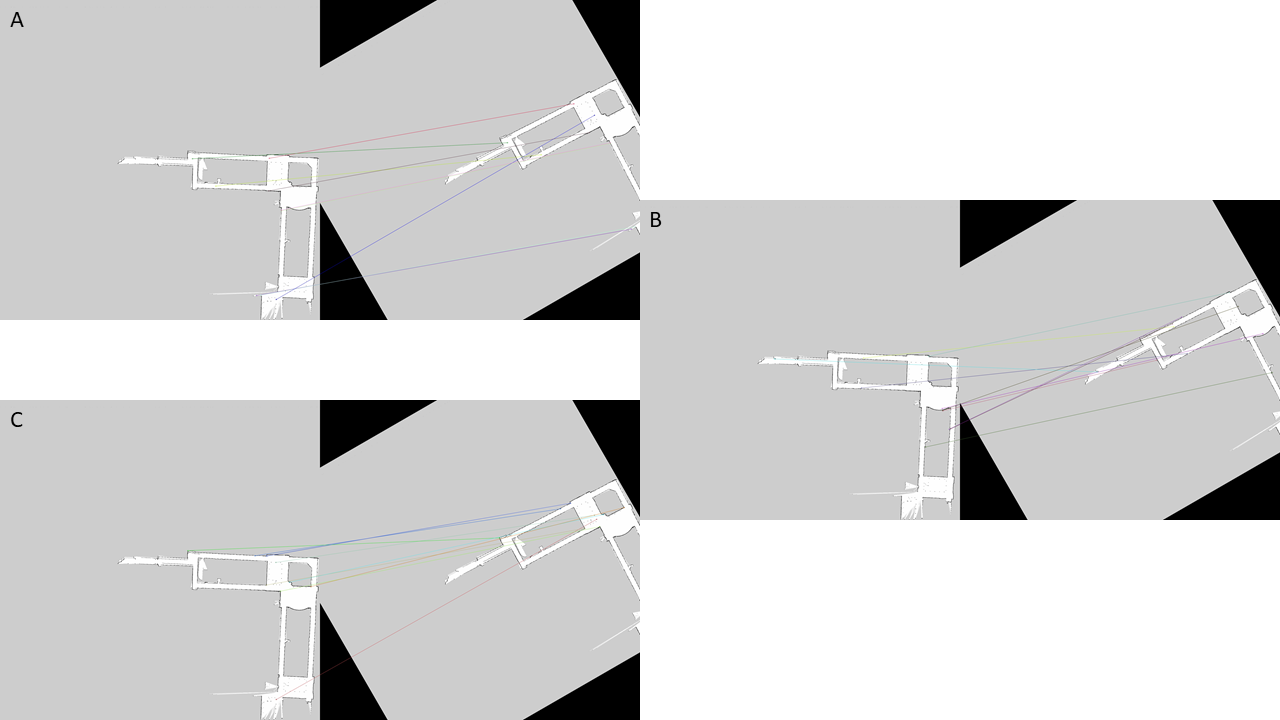
\includegraphics[width=1\textwidth]{figs/matching_of_30_rotation.png}
%----------------------------------------------------
    \caption{ The matching of 30$^\circ$ rotation images using (a) SIFT (b) SURF(c) ORB.}
%----------------------------------------------------
    \label{fig:rotation}
%----------------------------------------------------
\end{figure}
%....................................................

%....................................................
\begin{table}[H]
\centering
\caption{Results of comparing the images with 30$^\circ$ rotation.}
\begin{tabular}{ | m{3em} | m{2cm} | m{1.5cm} | m{1.5cm} | m{1.5cm} | m{3cm} | } 
\hline
& \textbf{Time(sec)} & \textbf{Kpnts1}  & \textbf{Kpnts2} & \textbf{Good Matches} & \textbf{Match Ratio}\\ 
\hline
\textbf{SIFT}  & 1.4 & 530 & 489 & 305 & 0.62\\ 
\hline
\textbf{SURF}  & 1.2 & 4503 & 5128 & 1370 & 0.30\\ 
\hline
\textbf{ORB}  & 0.39 & 500 & 500 & 280 & 0.56\\ 
\hline 
\end{tabular}
\label{table:rotation}
\end{table}


\begin{table}[H]
\centering
\caption{Matching ratio versus the rotation angle.}
\begin{tabular}{ | m{5em} | m{1cm} | m{1cm} | m{1cm} | m{1cm} | m{1cm} | m{1cm} | m{1cm} || m{1.6cm} | } 
\hline
\textbf{Angle $\rightarrow$} & \textbf{0$^\circ$} & \textbf{30$^\circ$} & \textbf{60$^\circ$} & \textbf{90$^\circ$} & \textbf{120$^\circ$} & \textbf{150$^\circ$} & \textbf{180$^\circ$} & \textbf{Average}  \\ 
\hline
\textbf{SURF} & 1 & 0.30 & 0.30 & 1 & 0.30 & 0.30 & 1 & 0.60 \\
\hline
\textbf{SIFT} & 0.95 & 0.62 & 0.63 & 0.92 & 0.63 & 0.65 & 0.90 & 0.90\\ 
\hline
\textbf{ORB} & 1 & 0.56 & 0.58 & 1 & 0.56 & 0.58 & 1 & 0.75 \\ 
\hline
\hline
%\textbf{Average} & 0.98 & 0.50 & 0.51 & 0.97 & 0.50 & 0.51 & 0.97 & 0.71 \\ 
%\hline
\end{tabular}
\label{table:rotationangle}
\end{table}

\subsubsection{Translation}
\label{sub:sec:translation}

In this investigation, $map_3$ is translated in steps of 200, with 0 being the control. The translated map is matched with the original map. The results are shown by Figure \ref{fig:translation}, Table \ref{table:translation} and Table \ref{table:translationchange}.

Table \ref{table:translation} shows that ORB is the fastest performing method followed by SIFT, and then SURF. Table \ref{table:translationchange}, shows that SURF as best performing method at match ratio of 0.99 followed closely by SIFT at 0.97. ORB has the lowest performance to varying translations, with a match ratio of 0.59.

\begin{figure}[H]
    \centering
    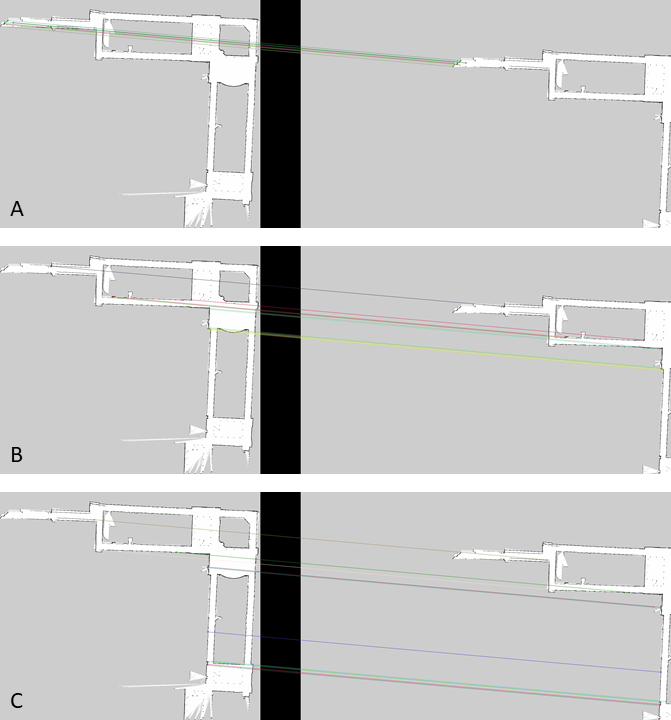
\includegraphics[width=1\textwidth]{figs/The_matching_of_translation_200.png}
    \caption{ The matching of translation(x:200 y:200) images using (a) SIFT (b) SURF (c) ORB.}
    \label{fig:translation}
\end{figure}

\begin{table}[H]
\centering
\caption{Results of comparing the images of translation in \ref{fig:translation}.}
\begin{tabular}{ | m{3em} | m{2cm} | m{1.5cm} | m{1.5cm} | m{1.5cm} | m{3cm} | } 
\hline
& \textbf{Time(sec)} & \textbf{Kpnts1}  & \textbf{Kpnts2} & \textbf{Good Matches} & \textbf{Match Ratio}\\ 
\hline
\textbf{SIFT}  & 3.23 & 530 & 285 & 278 & 0.98\\ 
\hline
\textbf{SURF}  & 3.79 & 4503 & 2598 & 2595 & 1\\ 
\hline
\textbf{ORB}  & 1.70 & 500 & 500 & 280 & 0.56\\ 
\hline
\end{tabular}
\label{table:translation}
\end{table}


\begin{table}[H]
\centering
\caption{Matching ratio versus the translation.}
\begin{tabular}{ | m{5.5em} | m{1cm} | m{1cm} | m{1cm} | m{1cm} | m{1cm} | m{1cm} || m{1.5cm} | m{1cm} | m{1cm} | m{1cm} | } 
\hline
\textbf{Translation $\rightarrow$} & \textbf{x:0 y:0} & \textbf{x:100 y:100}  & \textbf{x:300 y:300}  & \textbf{x:500 y:500} & \textbf{x:700 y:700} & \textbf{x:900 y:900} & \textbf{Average}   \\ 
\hline
\textbf{SIFT}  & 0.95 & 0.95 & 0.99 & 0.98 & 0.99 & 0.97 & 0.97 \\ 
\hline
\textbf{SURF}  & 1 & 0.99 & 0.99 & 0.99 & 0.99 & 0.99 & 0.99 \\ 
\hline
\textbf{ORB}  & 1 & 0.66 & 0.52 & 0.49 & 0.47 & 0.41 & 0.59 \\ 
\hline
\hline
%\textbf{Average}  & 0.98 & 0.87 & 0.83 & 0.82 & 0.82 & 0.79 & 0.85 \\ 
%\hline
\end{tabular}
\label{table:translationchange}
\end{table}


\subsubsection{Scaling}

In this investigation, $map_3$ is scaled in steps of 0.2. The scaled map is matched with the original map. The results are shown by Figure \ref{fig:scaling}, Table \ref{table:scaling} and Table \ref{table:scalingchange}. 

Table \ref{table:scaling} shows that for a scaling operation of 0.4, ORB is the fastest followed by SIFT then SURF. Furthermore, SIFT has the highest match ratio of 0.88 at a scale of 0.4, followed by SURF, then ORB.

Now Table \ref{table:scalingchange}, show the match ratio at multiple scales, which presents SIFT at the best overall performing method, with a match ratio of 0.82. Followed by SURF at 0.67, then ORB at 0.49.


\begin{figure}[H]
    \centering
    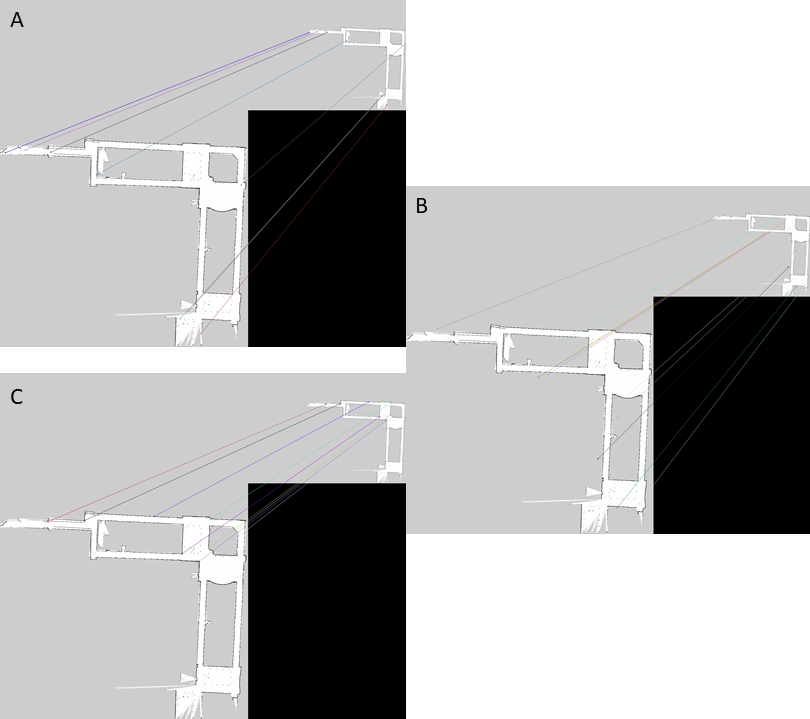
\includegraphics[width=1\textwidth]{figs/The_matching_of_scale_0_4.png}
    \caption{ The matching of varying scaling images using (a) SIFT (b) SURF (c) ORB.}
    \label{fig:scaling}
\end{figure}

\begin{table}[H]
\centering
\caption{Results of comparing the images with 0.4 scaling.}
\begin{tabular}{ | m{3em} | m{2cm} | m{1.5cm} | m{1.5cm} | m{1.5cm} | m{3cm} | } 
\hline
& \textbf{Time(sec)} & \textbf{Kpnts1}  & \textbf{Kpnts2} & \textbf{Good Matches} & \textbf{Match Ratio}\\ 
\hline
SIFT  & 1.05 & 530 & 84 & 74 & 0.88\\ 
\hline
SURF  & 1.35 & 4503 & 1013 & 671 & 0.66\\ 
\hline
ORB  & 0.29 & 500 & 496 & 208 & 0.42\\ 
\hline
\end{tabular}
\label{table:scaling}
\end{table}


\begin{table}[H]
\centering
\caption{Matching ratio versus the scaling.}
\begin{tabular}{ | m{5em} | m{1cm} | m{1cm} | m{1cm} | m{1cm} | m{1.5cm} | } 
\hline
\textbf{Scaling $\rightarrow$} & \textbf{0.2} & \textbf{0.4} & \textbf{0.6} & \textbf{0.8} & \textbf{Average} \\ 
\hline
\textbf{SIFT}  & 0.81 & 0.88 & 0.85 & 0.76 & 0.82 \\ 
\hline
\textbf{SURF}  & 0.68 & 0.66 & 0.67 & 0.66 & 0.67 \\ 
\hline
\textbf{ORB}  & 0.39 & 0.42 & 0.52 & 0.65 & 0.49 \\ 
\hline
\hline
%\textbf{Average}  & 0.62 & 0.65 & 0.68 & 0.69 & 0.66 \\
%\hline
\end{tabular}
\label{table:scalingchange}
\end{table}

\subsubsection{Noisy maps}
In this investigation, $map_3$ has salt and pepper noise applied at steps of 0.01. The modified image is then matched with the original image. The results are shown by Figure \ref{fig:noise}, Table \ref{table:noise} and table\ref{table:noisechange}. 

Table \ref{table:noise} shows match ratio and computation time at 3$\%$ noise, where ORB has the fastest computation time at 4.82 seconds followed by SIFT at 7.92 seconds, and SURF at 35.02 seconds close to ten times that of ORB.

Now Table \ref{table:noise} shows the match ratio of the different methods at steps of 0.01 noise. SIFT is best performing with an average of 0.83 match ratio followed by ORB at a 0.67 match ratio, and then SURF at a 0.61 match ratio.

\begin{figure}[H]
    \centering
    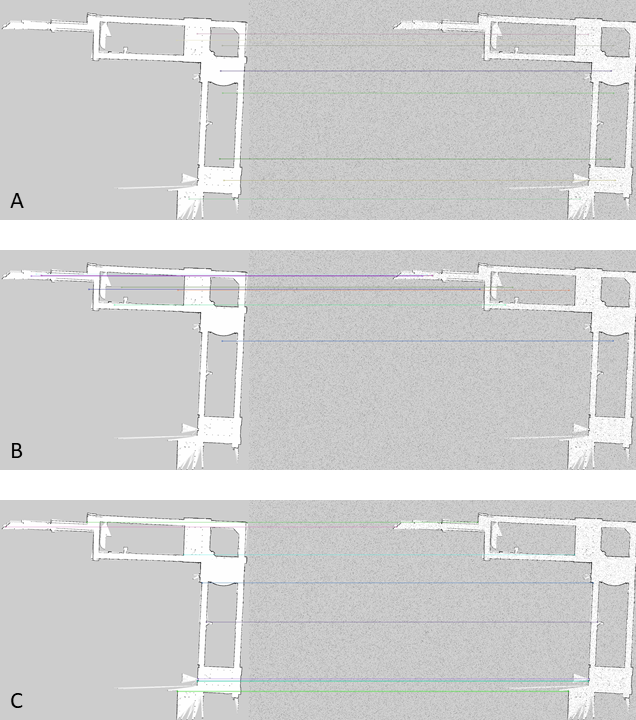
\includegraphics[width=1\textwidth]{figs/The_matching_of_noise_0_03.png}
    \caption{ The matching of 0.03 salt and pepper noise on varying images using (a) SIFT (b) SURF (c) ORB.}
    \label{fig:noise}
\end{figure}

\begin{table}[H]
\centering
\caption{Results of comparing the images with 0.03 salt and pepper noise.}
\begin{tabular}{ | m{3em} | m{2cm} | m{1.5cm} | m{1.5cm} | m{1.5cm} | m{3cm} | } 
\hline
& \textbf{Time(sec)} & \textbf{Kpnts1}  & \textbf{Kpnts2} & \textbf{Good Matches} & \textbf{Match Ratio}\\ 
\hline
\textbf{SIFT}  & 7.92 & 530 & 13436 & 441 & 0.83\\ 
\hline
\textbf{SURF}  & 35.02 & 4503 & 115422 & 2105 & 0.47\\ 
\hline
\textbf{ORB}  & 4.82 & 500 & 500 & 311 & 0.62\\ 
\hline
\end{tabular}
\label{table:noise}
\end{table}


\begin{table}[H]
\centering
\caption{Matching ratio versus the noise.}
\begin{tabular}{ | m{5em} | m{1cm} | m{1cm} | m{1cm} | m{1cm} | m{1cm} | m{1cm} | m{1cm} | m{1cm} | m{1cm} | m{1cm} | } 
\hline
\textbf{Noise $\rightarrow$ }& \textbf{0.01} & \textbf{0.02} & \textbf{0.03} & \textbf{0.04} & \textbf{Average} \\ 
\hline
\textbf{SIFT}  & 0.82 & 0.82 & 0.83 & 0.83 & 0.83 \\ 
\hline
\textbf{SURF}  & 0.76 & 0.65 & 0.55 & 0.47 & 0.61 \\ 
\hline
\textbf{ORB}  & 0.74 & 0.67 & 0.63 & 0.62 & 0.67  \\ 
\hline
\hline
%\textbf{Average}  & 0.78 & 0.72 & 0.67 & 0.64 & 0.70  \\ 
%\hline
\end{tabular}
\label{table:noisechange}
\end{table}

%====================================================
\subsubsection{Method selection summary}
%----------------------------------------------------

In this section, three different feature detection methods are compared similarly to work done in \cite{Karami2015}, with different translation and deformation such as scaling, rotation, noise and translation. For purposes of the work in this thesis, these transformations were applied to an occupancy grid map produced for this work. The results present display matching evaluation parameters such as the number of key-points, match ratio and the execution time for each method. 

The results show that ORB is the fastest, while SIFT performs the best in most scenarios. For exceptional cases when rotation angle is in steps of 90 degrees ORB and SURF outperform SIFT, these results match those of \cite{Karami2015}. In translation operations, SIFT and SURF perform similarly. Unlike results in \cite{Karami2015} ORB and SIFT do not show similar performance in noisy maps. In noisy maps, SURF's execution time is close to ten times the performance of ORB. In conclusion, SIFT is the most consistent in producing match ratios larger 0.80 for all the transformations and deformations. Therefore, SIFT will be used in this thesis because it has superior accuracy, and the time cost is not too high compared to SURF and ORB.


%====================================================
\section{Summary}
%----------------------------------------------------

In this chapter, the map merging problem was firstly defined, followed by investigating the literature around map merging. From the literature, image registration modules are discussed. Finally, image registration feature detectors SIFT, SURF and ORB are investigated to find the optimal methods for application in this thesis. The investigation is conducted due to the lack of literature comparing the methods in an occupancy grid map merging application. In the next chapter implementation of multi-robot, multi-session and multi-resolution map merging is discussed and described.




%\section{Notation and definition}
%
%The maps are assumed to be a 2D occupancy grid map \(m\) which is a matrix of N x M. Given two maps \(m_1\) and \(m_2\), which are 2D occupancy grid maps. We need to find the relative transformation(rotation and translation) between the maps. Let 2x1 translation vector  \(T\)  and 2 x 2 rotation matrix \(R_{\theta}\) be:

%\begin{equation}
%R_{theta} =  \begin{bmatrix}
%\cos(\theta) & -\sin(\theta)  \\
%sin(\theta) & \cos(\theta)
%\end{bmatrix} ,T =  \begin{bmatrix}
%\delta_{x}  \\
%\delta_{y}
%\end{bmatrix} 
%\end{equation}.

%Assuming the task is to merge \(m_2\) into \(m_1\), the map merging objective is to find \(R\) and \(T\) such that the transformed \(m_2\) which is \(m_{2}^{'}\) , overlaps with \(m_1\). The following equation is a defines a verification index which is maximized according to transformation \(R\) and \(T\) : 

%\begin{equation}
%(R_\theta, T) = argmax V(m_1 , m_{2}^{'})
%\end{equation}.

%The criterion \(V(\cdot)\) is used to evaluate the map merging process, such as a similarity index in (Birk and Capin, 2006).









%(Howard, 2006) use to prove that it is essential to choose the best SLAM algorithm to solve the map merging problem











